\documentclass[a4paper]{article}
\usepackage[utf8]{inputenc}
\usepackage[spanish, es-tabla, es-noshorthands]{babel}
\usepackage[table,xcdraw]{xcolor}
\usepackage[a4paper, footnotesep = 1cm, width=20cm, top=2.5cm, height=25cm, textwidth=18cm, textheight=25cm]{geometry}
%\geometry{showframe}

\usepackage{tikz}
\usepackage{amsmath}
\usepackage{amsfonts}
\usepackage{amssymb}
\usepackage{float}
\usepackage{graphicx}
\usepackage{caption}
\usepackage{subcaption}
\usepackage{multicol}
\usepackage{multirow}
\setlength{\doublerulesep}{\arrayrulewidth}
\usepackage{booktabs}
\usepackage{mathrsfs,amsmath}
\usepackage{hyperref}
\hypersetup{
    colorlinks=true,
    linkcolor=blue,
    filecolor=magenta,      
    urlcolor=blue,
    citecolor=blue,    
}

\newcommand{\quotes}[1]{``#1''}
\usepackage{array}
\newcolumntype{C}[1]{>{\centering\let\newline\\\arraybackslash\hspace{0pt}}m{#1}}
\usepackage[american]{circuitikz}
\usetikzlibrary{calc}
\usepackage{fancyhdr}
\usepackage{units} 

\graphicspath{./Imagenes}

\pagestyle{fancy}
\fancyhf{}
\lhead{22.05 ASSD}
\rhead{Mechoulam, Lambertucci, Rodriguez, Londero}
\rfoot{Página \thepage}

\begin{document}

%%%%%%%%%%%%%%%%%%%%%%%%%
%		Caratula		%
%%%%%%%%%%%%%%%%%%%%%%%%%

\begin{titlepage}
\newcommand{\HRule}{\rule{\linewidth}{0.5mm}}
\center
\mbox{\textsc{\LARGE \bfseries {Instituto Tecnológico de Buenos Aires}}}\\[1.5cm]
\textsc{\Large 22.05 Análisis de Señales y Sistemas Digitales}\\[0.5cm]


\HRule \\[0.6cm]
{ \Huge \bfseries Trabajo práctico N$^{\circ}$2}\\[0.4cm] 
\HRule \\[1.5cm]


{\large

\emph{Grupo 3}\\
\vspace{3px}

\begin{tabular}{lr} 	
\textsc{Mechoulam}, Alan  &  58438\\
\textsc{Lambertucci}, Guido Enrique  & 58009 \\
\textsc{Rodriguez Turco}, Martín Sebastian  & 56629 \\
\textsc{Londero Bonaparte}, Tomás Guillermo  & 58150 \\
\end{tabular}

\vspace{20px}

\emph{Profesores}\\
Jacoby, Daniel Andres\\
Belaustegui Goitia, Carlos F.\\
Iribarren, Rodrigo Iñaki\\
\vspace{3px}
%\textsc{} \\	

\vspace{100px}

\begin{tabular}{ll}

Presentado: & 15/05/20\\

\end{tabular}

}

\vfill

\end{titlepage}



%%%%%%%%%%%%%%%%%%%%%
%		Informe		%
%%%%%%%%%%%%%%%%%%%%%

\section*{Ejercicio 1}
\begin{itemize}
	\item[d)] $\mathbf{R \left[ x \left( nT \right) \right] = 5nT x^2 \left( nT \right)}$ 
	
		\textbf{Invariancia:}
		
		$R \left[ x \left( nT - \alpha \right) \right] = 5nT x^2 \left( nT - \alpha \right)$ 
		
		$T \left[ R \left[ x \left( nT \right) \right] \right] = T \left[ 5nT x^2 \left( nT \right) \right] = 5(nT-T) x^2 \left( nT - \alpha \right)$ 
		
		No es tiempo invariante.
		
		\textbf{Causalidad:} Es causal ya que no depende de entradas futuras.
		
		\textbf{Linealidad:}
		
		 $R \left[ ax_1 \left( nT \right) + bx_2 \left( nT \right) \right] = 5nT \left(a{x_{1}}^{2} + b {x_{2}^{2}}\right) \left( nT \right) \neq aR \left[ x_1 \left( nT \right) \right] + bR \left[ x_2 \left( nT \right) \right]$

		No es un sistema lineal.
		
	\item[e)] $\mathbf{R \left[ x \left( nT \right) \right] = 3x \left( nT + 3T\right)}$ 
	
		\textbf{Invariancia:}
		
		$R \left[ x \left( nT - T \right) \right] = 3x \left( nT + 3T - \alpha \right)$ 
		
		$T \left[ R \left[ x \left( nT \right) \right] \right] = T \left[ 3x \left( nT + 3T \right) \right] = 3x \left( nT + 3T - \alpha \right)$ 
		
		Es tiempo invariante.
		
		\textbf{Causalidad:} No es causal ya que depende de entradas futuras.
		
		\textbf{Linealidad:}
		
		 $R \left[ ax_1 \left( nT \right) + bx_2 \left( nT \right) \right] = 3 \left[ ax_{1} \left( nT + 3T \right) + b x_{2} \left( nT + 3T \right) \right] = a 3 x_{1} \left( nT + 3T \right) + b 3x_{2} \left( nT + 3T \right) = aR \left[ x_1 \left( nT \right) \right] + bR \left[ x_2 \left( nT \right) \right]$

		Es un sistema lineal.
		
	\item[i)] $\mathbf{R \left[ x \left( nT \right) \right] = x \left( nT + T\right) e^{-nT}}$ 
	
		\textbf{Invariancia:}
		
		$R \left[ x \left( nT - \alpha \right) \right] =  x \left( nT + T - \alpha  \right) e^{-nT}$ 
		
		$T \left[ R \left[ x \left( nT \right) \right] \right] = T \left[  x \left( nT + T - \alpha \right) e^{-nT + \alpha} \right] = x \left( nT + T -\alpha \right) e^{-nT + \alpha}$ 
		
		No es tiempo invariante.
		
		\textbf{Causalidad:} No es causal ya que depende de entradas futuras.
		
		\textbf{Linealidad:}
		
		 $R \left[ ax_1 \left( nT \right) + bx_2 \left( nT \right) \right] = \left[ a x_{1} \left( nT \right) + b x_{2} \left( nT \right) \right] e^{-nT + T} = a x_{1} \left( nT \right) e^{-nT + T} + b x_{2} \left( nT \right) e^{-nT + T} = aR \left[ x_1 \left( nT \right) \right] + bR \left[ x_2 \left( nT \right) \right]$

		Es un sistema lineal.		

\end{itemize}

\section*{Ejercicio 2b}
La ecuación en diferencia del sistema se vale de la función auxiliar $e(nT)$.

\begin{enumerate}
	\item	$e(nT) = x(nT) + e(nT - T) - 0.5e(nT - 2T)$
	\item	$y(nT) = e(nT) + e(nT - T)$
\end{enumerate}

\section*{Ejercicio 9}
La ecuación en diferencia del sistema es
\begin{equation*}
	y(nT) = 0.5x(nT - 2T) + \alpha y(nT - T) + \beta y(nT - 2T)
\end{equation*}

De esta formase obtienen los siguientes resultados.

\begin{figure}[H]
\centering
\begin{subfigure}{.49\textwidth}
\centering
	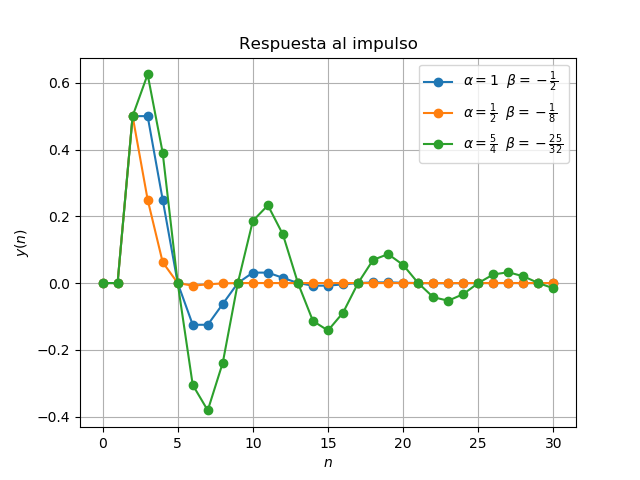
\includegraphics[width=\textwidth]{Imagenes/9-impulso.png}
\end{subfigure}
\begin{subfigure}{.49\textwidth}
\centering
	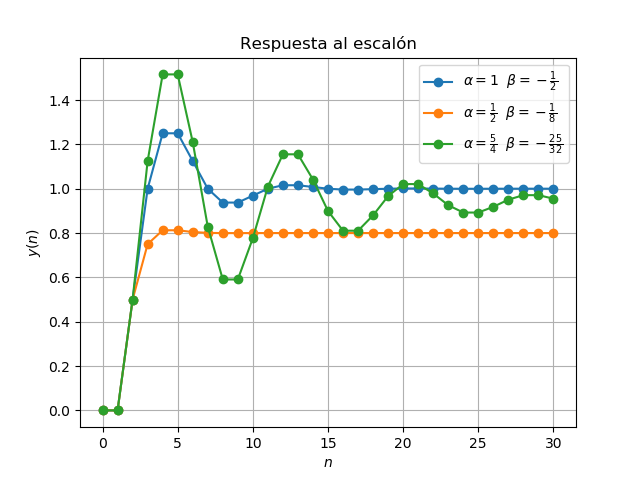
\includegraphics[width=\textwidth]{Imagenes/9-escalon.png}
\end{subfigure}
\end{figure}

Se puede determinar la frecuencia de oscilación para los casos de $\alpha = 1$ y $\beta = -\frac{1}{2}$ y $\alpha = \frac{5}{4}$ y $\beta = -\frac{25}{32}$, tanto de la respuesta al impulso como del escalón. Para todos los casos se obtiene $f_o = \frac{125}{T}$.
\begin{center}
	\textcolor{red}{\textbf{Para estimar la respuesta en frecuenacia en el caso de a...}}
\end{center}

\section*{Ejercicio 11}
La ecuación en diferencia del sistema es: %(con $T=1 \ ms$)
\begin{equation*}
	y(n) = 0.4 y(n - 1) + 0.4 x(n)
\end{equation*}

Siendo este un sistema relajado, se busca $y(n)$ con $x(n) = \delta (n)$:
\begin{equation*}
	h(0) = 0.4 x(0) + 0.4h(-1) = 0.4
\end{equation*}
\begin{equation*}
	h(1) = 0.4 x(1) + 0.4h(0) = 0.4^2
\end{equation*}
\begin{equation*}
	h(2) = 0.4 x(2) + 0.4h(1) = 0.4^3
\end{equation*}
\begin{equation*}
	...
\end{equation*}
\begin{equation*}
	h(n) = 0.4^{n+1}
\end{equation*}

Se busca que la salida quede expresada de la forma:
\begin{equation*}
	y(n) = y_{zi}(n) + y_{zs}(n)
\end{equation*}

Donde
\begin{equation*}
	\lim_{n\to\infty} y(n) = \lim_{x\to\infty} y_{zi}(n) + y_{zs}(n) \longrightarrow h(n)*x(n) + 0
\end{equation*}

Asumiendo excitación senoidal $x(nt) = cos(n \omega T) = \frac{e^{j n \omega T}}{2j} + \frac{e^{-j n \omega T}}{2j}$
\begin{equation*}
	y(nT) = R[x(nT)] = \frac{1}{2j} R\left[ e^{j n \omega T} \right] + \frac{1}{2j} R\left[ e^{-j n \omega T} \right] = \frac{1}{2j} y_1 (\omega T) + \frac{1}{2j} y_2 (\omega T)
\end{equation*}

Tomando
\begin{equation*}
	y_1 (\omega T) = \sum_{k=0}^{n} x_1(n - k) h(k) = \sum_{k=0}^{n}e^{j \left( n - k \right) \omega T } 0.4^{n+1} = 0.4 \sum_{k=0}^{n}e^{j \left( n - k \right) \omega T } e^{ln \left( 0.4 \right) } = 0.4 e^{j n \omega T } \sum_{k=0}^{n}e^{j \left( - k \right) \omega T \ ln \left( 0.4 \right) }
\end{equation*}

Sabiendo que es una serie geométrica
\begin{equation*}
	y_1 (\omega T) = 0.4 e^{j n \omega T } \frac{ e^{ \left[ ln \left( 0.4 \right) - j k \omega T \right] \left(n + 1 \right) } - 1}{e^{ ln \left( 0.4 \right) - j k \omega T} - 1}
\end{equation*}
\begin{equation*}
	\lim_{n\to\infty} y_1 (n) = e^{j n \omega T } \frac{0.4}{1 - e^{ ln \left( 0.4 \right) - j k \omega T}} = \tilde{y}_1(n)	
\end{equation*}
\begin{equation*}
	H(j \omega) = \frac{0.4}{1 - e^{ ln \left( 0.4 \right) - j k \omega T}}	
\end{equation*}

Siendo así:
\begin{equation}
	|H(j \omega)| = \frac{0.4}{\sqrt{1 + 0.4^2 - 0.8 cos( \omega T)}}
	\label{equ:mod}	
\end{equation}
\begin{equation}
	\phase{H(j \omega)} = arctan \left( \frac{0.4 sen( \omega T)}{0.4 cos( \omega T) - 1} \right)
\end{equation}

\begin{figure}[H]
\centering
\begin{subfigure}{.49\textwidth}
\centering
	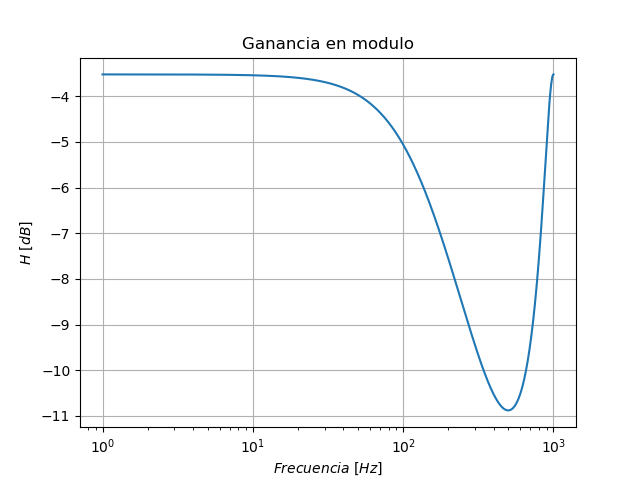
\includegraphics[width=\textwidth]{Imagenes/11-modulo.png}
\end{subfigure}
\begin{subfigure}{.49\textwidth}
\centering
	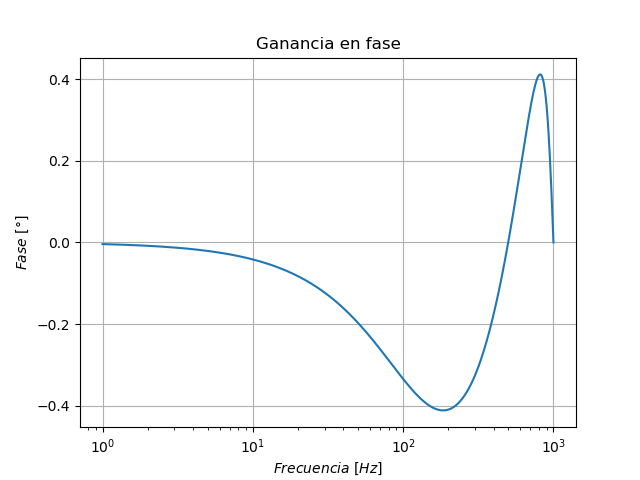
\includegraphics[width=\textwidth]{Imagenes/11-fase.png}
\end{subfigure}
\end{figure}

Evaluando (\ref{equ:mod}) en 0, se obtiene $H(0) = \frac{2}{3}$. Ahora se busca la frecuencia tal que $|H(j \omega)| = \frac{2}{3 \sqrt{2}}$. Despejando, se obtiene $f = \frac{0.99}{2 \pi T} = 157.31 \ Hz$.

\end{document}